\chapter{Graphical Representations} 

After parsing the Blazon sentence into a parse tree the application attempts to draw a visual representation of the shield.  This is done via the use of HTML5's Canvas element and JavaScript.  

Producing the Graphical Depiction of the Blazon was less important from a  functionality standpoint than correct parsing of sentences but does make for a much more interesting application for an end user.  


\section{Adding a Graphical Description to Data Structures}
The logical way to draw the shield was to approach the task in the same way as the textual description is handled.  Each of the data structures acting as nodes in the parse tree were expanded to implement a draw function which was called on each node in the parse tree as it was navigated. 


This approach provided several advantages.  Firstly it utilised the parse tree and data structures which were all ready implemented, working and fully tested.  Secondly it provided a way to continue working in iterative stages like the rest of the application and thirdly if it provided the potential for very generic drawing functions that would provide a lot of reuse.


Once again the most challenging aspect in the implementation were the semi formal charges.  The decision was made to ask the user to provide an image of the semi-formal charge they wanted to define.  This image would then be loaded directly onto the canvas in the appropriate place.  Due to the time constrains on development time this was never implemented which a large limitation of the application.




\section{Drawing a Shield}

The first stage in implementing a graphical front end to the application was to define a way of drawing a shield.  this was achieved by utilising the Canvas element's path functions.  


The equation for the curve of the shield was:


\begin{figure}[H]
$$ y = 625- x^2/500  $$
\caption{For x =-300 through to x =+300}
\label{math:curve}
\end{figure}


One of the quirks of HTML5's Canvas is that the y axis is inverted.  The top left corner of the Canvas is (0,0).  Which is why there is a negative constant in the parabola defined in \ref{math:curve}.  The rest of the shield is defined as a path from the end of the parabola in a rectangle back to the other edge of the parabola.

The whole area is now clipped which is another function provided by Canvas that ensures no drawing can occur outside of the current path, the shield. 


\section{Drawing Tinctures}
{
	
One the actual body of the shield was drawn the next step was to implement the draw functions of Tinctures as they are the most basic elements of Blazon.  It would be very hard to test either Charges or Line Types without Tinctures being defined before hand.

Tincture objects all needed to have hex colours defined for them which was a simple addition to the constructor.  The draw function was then defined as a generic function that took a path on the Canvas and used the given Canvas function \emph{fill} to colour the bounded area in the colour of the hex colour.  

}

\section{Partitioning Fields}

Successfully partitioning fields in the graphical representation was one of the more challenging aspects of the project for several reasons.


Any field can be partitioned by any partition therefore all the partition calculations need to be completely generic so that they can be used in all the possible situations that may arise.  This causers a large number of edge cases to occur. 

Every field needs to have consistent winding, the order the points that compose the field are joined together, so that the top left ordering of Blazon isn't lost.


\section{Implementing Field Partitioning}

What needs to be achieve is a system that takes the boundaries of a field and a partition and turns this into a series of new boundaries depending upon the partition given. 


The algorithm I devised for partitioning a field takes the boundaries of the current field and places the current partition onto it.   The algorithm then determines all the points of intersection between the field boundaries and the partition.  

The points of intersection need to be grouped together in a way to generate new boundaries of the sub fields formed from the partition.  

If a point of intersection lies between two corner points of the boundary then it becomes a corner of the new fields.  If an intersection occurs upon a corner of the current boundaries then it is present in both sets of boundaries generated for the new field. 


\emph{A function that takes the boundary of the current field, the lines of partition determined by the current partition and the number of sub fields to be produced:}

\begin{figure}[H]
\begin{algorithmic}

\STATE $2dPoint[] \, Boundary$
\STATE $2dPoint[] \, lines\, of\, Partition$
\STATE $int\, NumberOfSubFields $ \\


\COMMENT{Create a two dimensional array, each element will hold a 2dPoint[] for the boundaries of a new sub-field}


\STATE $New Fields = new Array$ 
\FOR{ Every new sub-field, $NumberOfSubFields$}
	\STATE $New Fields[]=new 2dPoint[]$
	
\ENDFOR

\end{algorithmic}
\end{figure}


\begin{figure}[H]
\begin{algorithmic}
\STATE $CurrentFieldIndex =0$
\FOR{Every point in $Boundary$}
	\STATE $NextPoint =$ the next point in $Boundary$

	\IF{ There an intersect between the current point and the next point}

		\IF{ The point of intersect lies on the current point in the boundary}
			
			\STATE  $NewFields[CurrentFieldIndex] = $ the point of intersect \COMMENT{Add the point of intersection to the current sub-field}
			\STATE $CurrentFieldIndex++$
	        \STATE $CurrentFieldIndex \%=NumberOfSubFields$\COMMENT{Instead of going out of bounds go back to zero}
	        \STATE $NewFields[CurrentFieldIndex] = $ the point of intersect \COMMENT{Add the point to the next sub-field} 
		
        \ELSIF{ The point of interest lies on $NextPoint$}
        	\STATE Ignore and deal with next loop iteration.
        \COMMENT {The intersect isn't on a corner}
        \ELSE

        	\STATE $NewFields[CurrentFieldIndex] = $ the current point in $Boundary$ \COMMENT{Add the current boundary point to the current sub-field}
        	\STATE $NewFields[CurrentFieldIndex] = $ the point of intersect \COMMENT{Add the point of intersection to the current sub-field}
			\STATE $CurrentFieldIndex++$
	        \STATE $CurrentFieldIndex \%=NumberOfSubFields$\COMMENT{Instead of going out of bounds go back to zero}
	        \STATE $NewFields[CurrentFieldIndex] = $ the point of intersect \COMMENT{Add the of intersection point to the next sub-field} 
		
		\ENDIF
	\ELSE
		\STATE $NewFields[CurrentFieldIndex] = $ the current point in $Boundary$ \COMMENT{Add the current boundary point to the current sub-field} \COMMENT {no intersection succoured}
	\ENDIF

\ENDFOR

\FOR{Every element if  $NewFields$}
	\STATE Set Winding \COMMENT {The boundaries must be defined so that the top left most point is the first in the array or the ordering of the fields becomes skewed} 

\STATE return $NewFields$
\ENDFOR
\end{algorithmic}
\caption{Pseudo code dividing a field into a number of sub-fields based upon a given partition.}
\label{fig:redsea}
\end{figure}


\section{A Visualisation}

What the algorithm in figure \ref{fig:redsea} is doing is dividing the field into a number of sub-fields.  This involves finding points of intersection between the partition and the field parameter.  A check needs to be made between each adjacent point of the boundary as to whether there is a point of intersection with the partition between them, if there is the the first point is assigned to the first sub-field and the second point to the second boundary with the point of intersection assigned to both. 

There  is an edge case where the point of intersection lies directly on one of the boundary points, in this case the point must belong to both sub-fields.  A visual example is provided in figure \ref{fig:bounds}.


\begin{figure}[H]
  \centering
    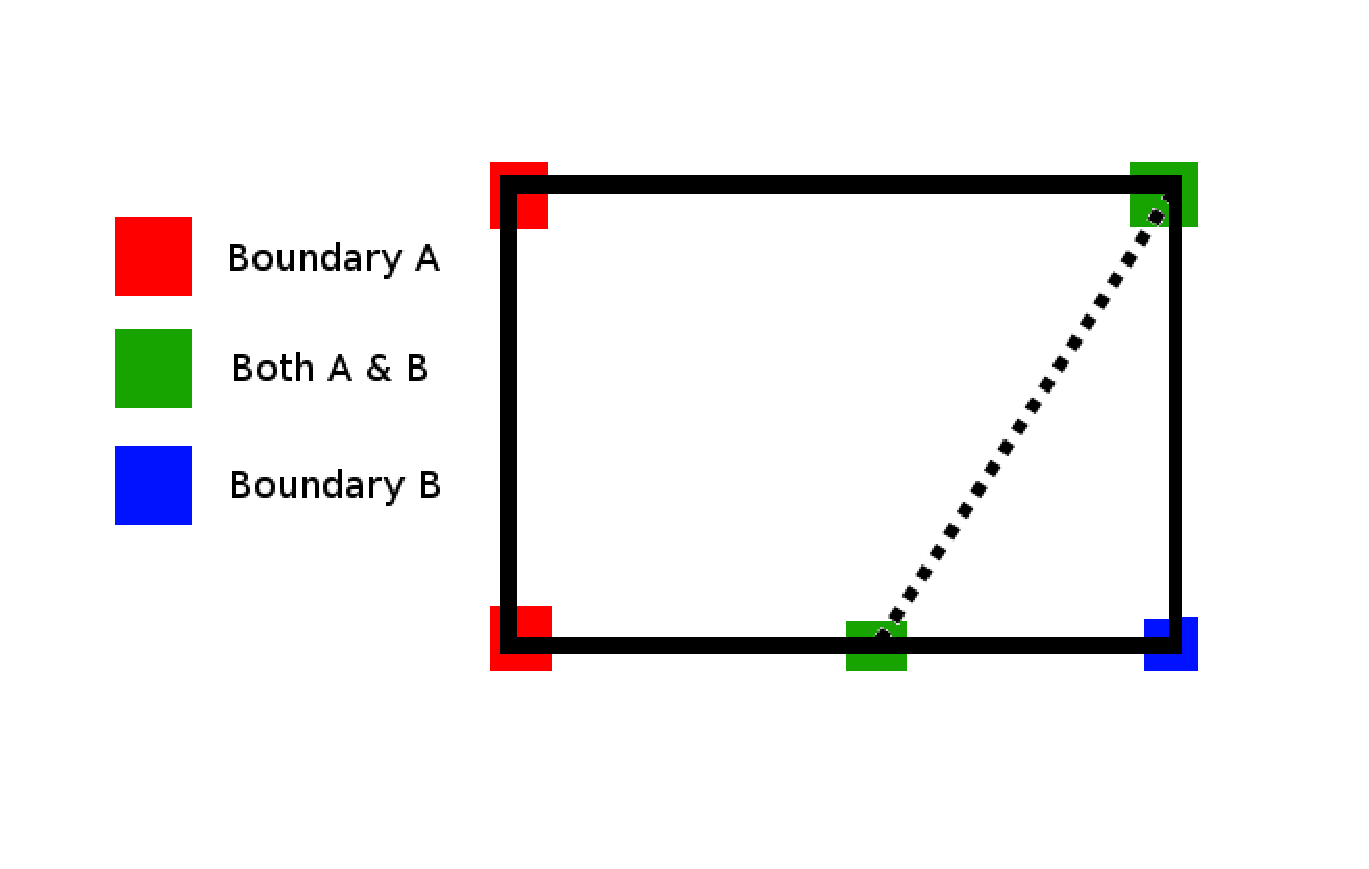
\includegraphics[width=\textwidth]{graphics/images/bounds.eps}
  \caption{UML description of a Tincture.}
  \label{fig:bounds}
  
\end{figure}

\section{Individual Partitions}
The only part section of graphically representing partitioning is defining how each partition is defined before being passed to the function in figure \ref{fig:redsea}.  Each partition is obviously different graphically and generally defining the line of intersection across a field was not too complex.

Bare in mind that these \emph{lines} are not drawn but are merely used to define paths and that the points of intersection are used to determine boundaries so defining a line across the entire canvas is fine as the excess is discarded. 

\subsection{Fess}
The line of intersection is defined across the entire canvas horizontally at the median Y axis value for the field. 
\subsection{Pall}
The line of intersection is defined across the entire canvas vertically at the median X axis value for the field. 
\subsection{Bend}
If the field is rectangular the line is simply defied to connect the top left to bottom right corners else the line of intersection is defined across the entire canvas at a forty five degree decline in such a way that the line intersects the median Y axis value for the field.
\subsection{Bend Sinister}
Exactly the same as above but at an incline instead of a decline.
\subsection{Cross}
A concatenation of Fess and Pall. The middle X and Y values are calculated for the field and then used for both Fess and Pall partitions.
\subsection{Saltire}
The same as Cross but with Bend and Bend Sinister instead of Fess and Pall.

\section{Implementing Charges}
The graphical implementation of Charges mirrored the implementation of each individual partition's line of intersection, see figure \ref{fig:charge} except instead of being a line a bar needed to be drawn instead.  

Presenting an appropriately scaled charge for the size of the field presented some of a challenge.  A thickness value for the charge was computed from the attributes of the field.  The thinness for a charge was defined as the lesser of either the difference in the maximum Y value for the field and the minimum Y value for the field or the equivalent on the X axis divided by three. 

\begin{figure}[H]
\subfigure[\emph{"A Field partitioned Per Bend."}]{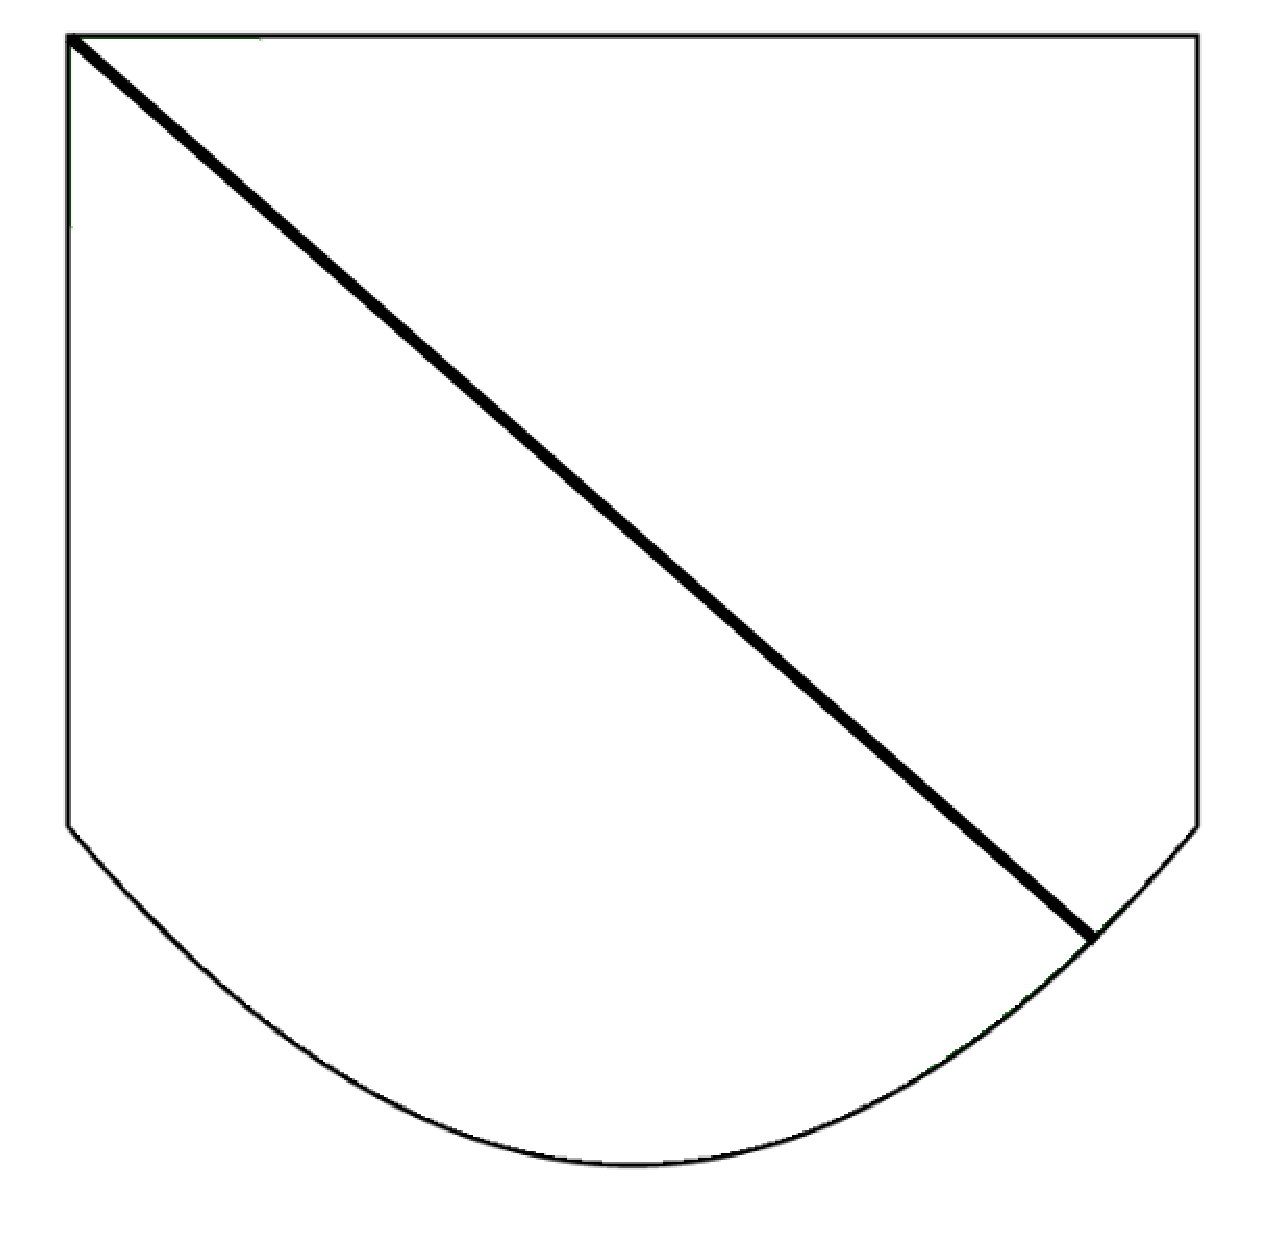
\includegraphics[width=0.5\textwidth]{graphics/images/bend.eps}}
\hfill
\subfigure[\emph{"A Field Charged Per Bend"}]{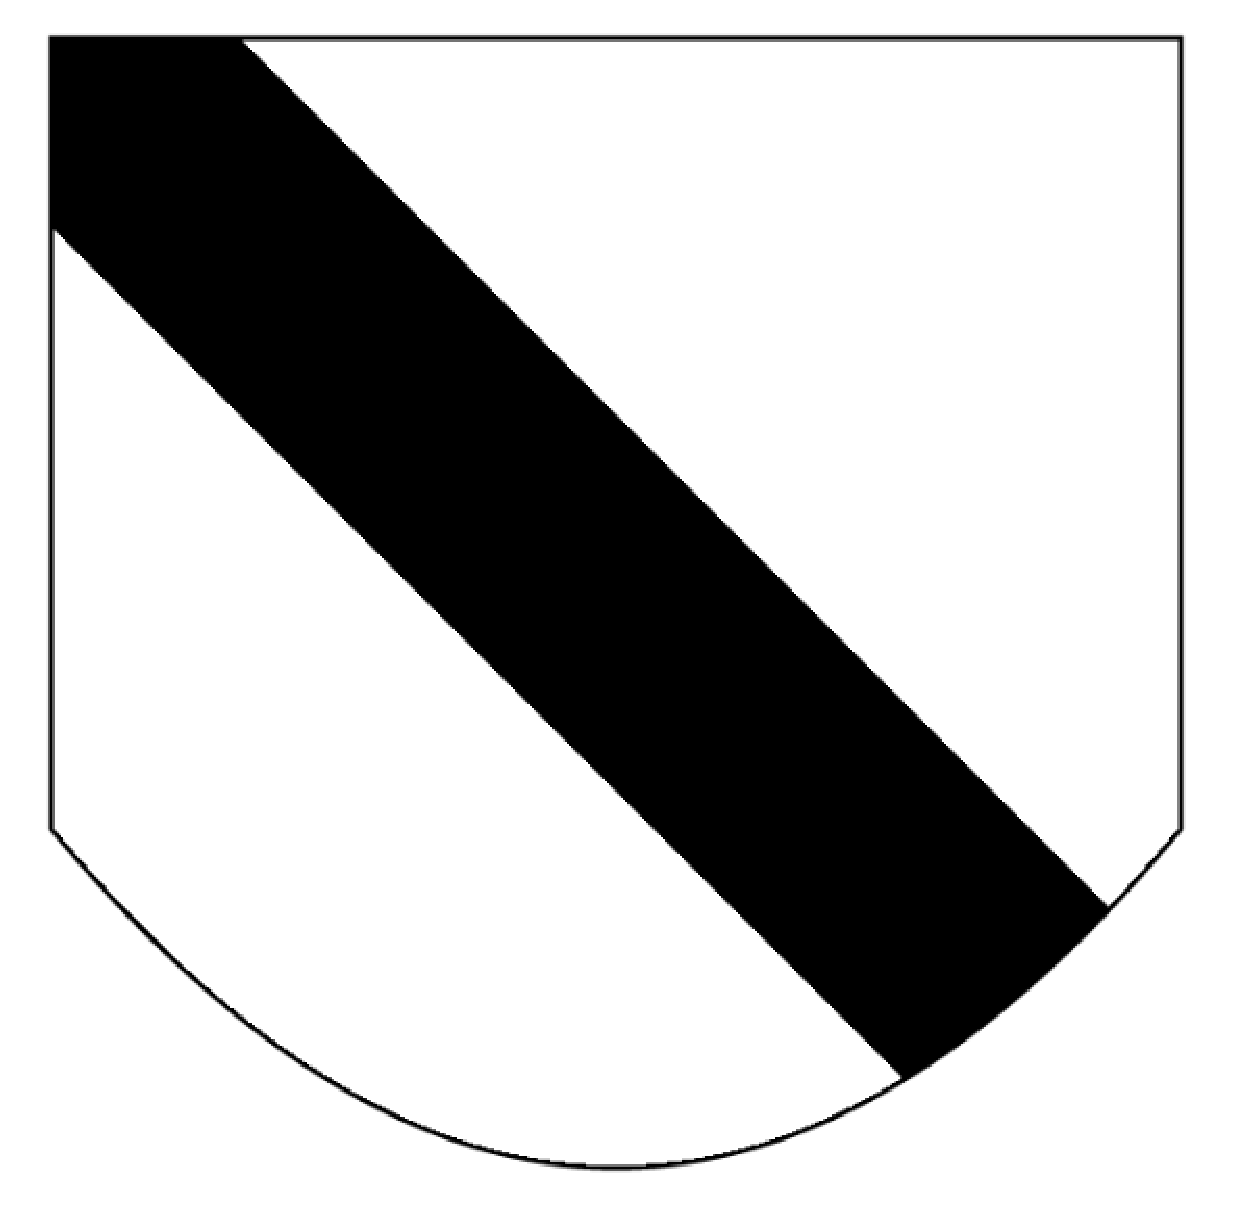
\includegraphics[width=0.5\textwidth]{graphics/images/bendcharge.eps}}
\hfill
\caption{The majority of the functionality for defining the line of partition for \emph{Bend} and the Charge \emph{Bend} is the same.}
\label{fig:charge}
\end{figure}


Only a little adapting was required to re-using the functionality from each Partitions definition to render a charge.  Firstly the intersection points needed to be calculated as before then these points were included in a Canvas path that included also used the intersect points plus and minus the thickness value.  This path was then passed to a Tinctures's Draw function and filled accordingly. 


\begin{figure}[H]
  \centering
    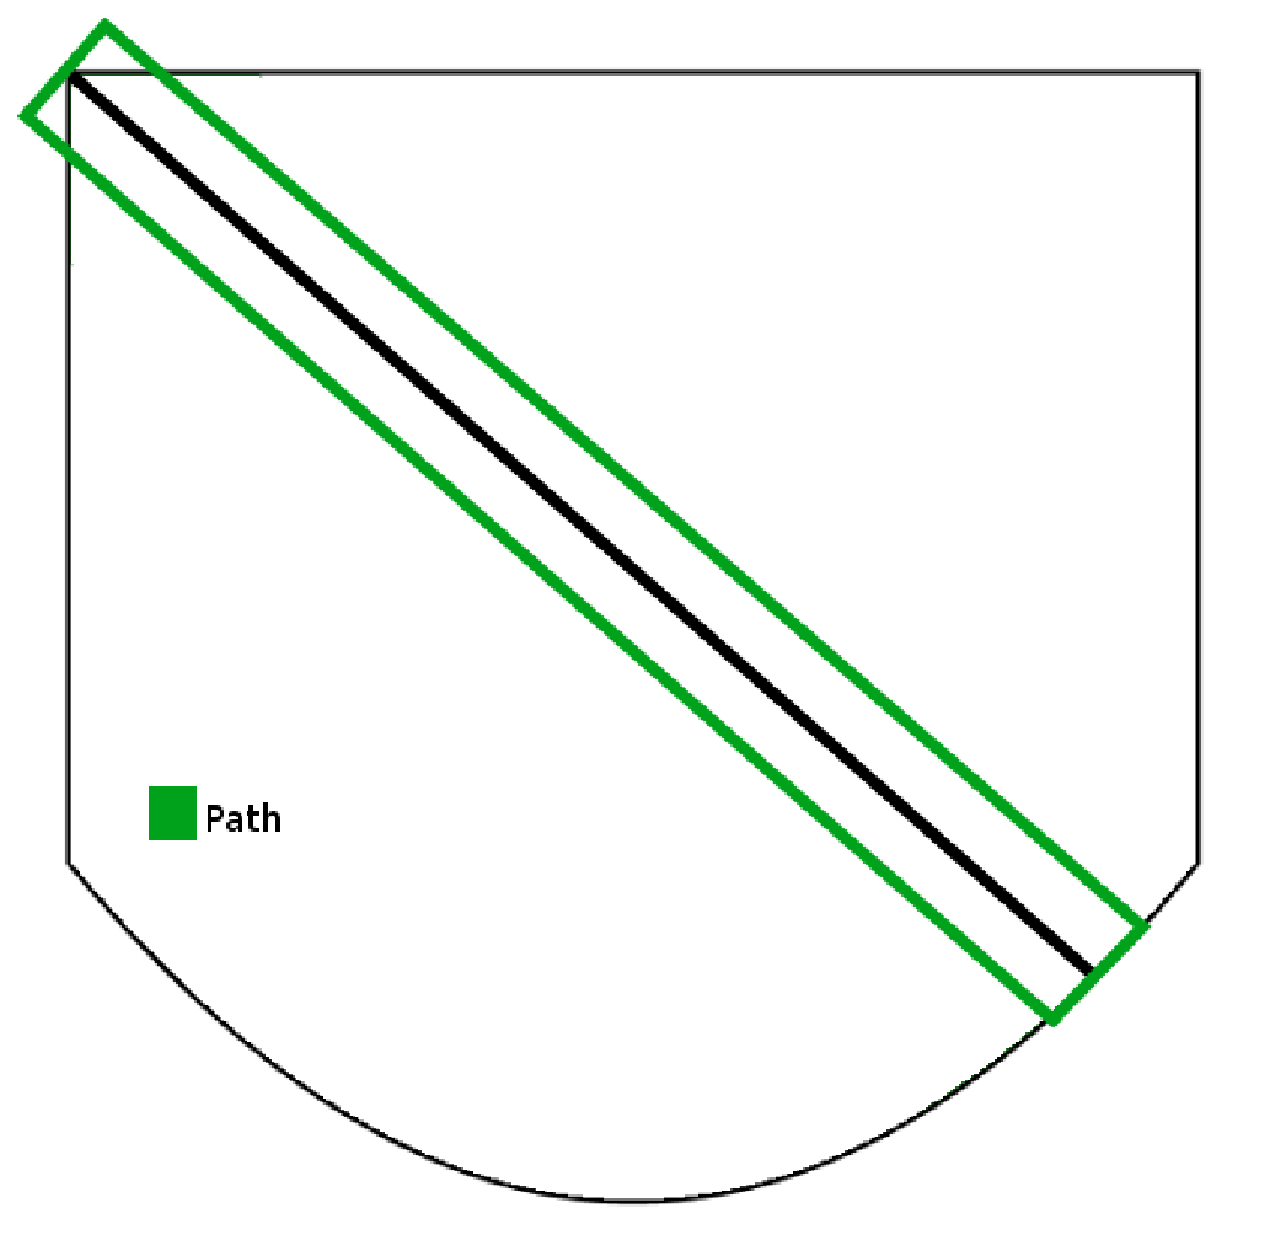
\includegraphics[width=\textwidth]{graphics/images/thickness.eps}
  \caption{A visualisation of defining a path offset from where the equivalent partition would be by a thickness}
  \label{fig:thickness}
  
\end{figure}


\section{A Third Party Library}
To calculate line intersections a third party library\cite{2dforyou} written by \emph{Kevin Lindsey} was utilised.  The library features a whole suit of useful functions for performing two dimensional geometry. The reasoning behind using a library over implementing the behaviour internally were sane as there were time constrains on the application development and the library has been actively maintained since 2002 which suggest a high likeliness that it is properly implement and tested.

























